% Springer classic template (svjour3)
\documentclass{svjour3}

\usepackage[utf8]{inputenc}
\usepackage[T1]{fontenc}
\usepackage{lmodern}
\usepackage{fix-cm}
\renewcommand{\rmdefault}{lmr}
\renewcommand{\sfdefault}{lmss}
\renewcommand{\ttdefault}{lmtt}
\usepackage{microtype}
\usepackage{silence}
\WarningFilter{latex}{Command \showhyphens has changed.}
\usepackage{amsmath,amssymb,mathtools}
\usepackage{booktabs}
\usepackage{enumitem}
\usepackage{graphicx}
\usepackage{tikz}
\usetikzlibrary{arrows.meta,positioning}
\usepackage{natbib}
\setcitestyle{authoryear,round}
\usepackage{xurl}
\usepackage[hidelinks]{hyperref}
\usepackage{orcidlink}

\title{Judgment Chain Linguistic Smart Contracts: Conditional Enforcement Semantics for Jailbreak-Resistant Language Models}
\titlerunning{Linguistic Smart Contracts for Language Models}

\author{Aryan Singh Chandel\,\orcidlink{0009-0007-1774-2480}}
\authorrunning{A. S. Chandel}

\institute{Aryan Singh Chandel \at
  RJIT (Rustamji Institute of Technology), Gwalior, India \\
  \email{aryansingh19gh@gmail.com}
}

\journalname{Preprint}
\date{June 26, 2026}

\makeatletter
\@ifundefined{definition}{\spnewtheorem{definition}{Definition}{\bfseries}{\rmfamily}}{}
\@ifundefined{assumption}{\spnewtheorem{assumption}{Assumption}{\bfseries}{\rmfamily}}{}
\@ifundefined{proposition}{\spnewtheorem{proposition}{Proposition}{\bfseries}{\itshape}}{}
\makeatother
\raggedbottom
\emergencystretch=2em

\begin{document}
\maketitle

\begin{abstract}
Prompt-level safety rules are often written as though they were enforceable constraints, even when they remain embedded in the very generation process they are meant to regulate. This paper proposes a stricter standard: a linguistic rule should count as a smart contract only when its trigger semantics and consequence semantics are externally evaluable, stable under paraphrase, and auditable under adversarial variation. We formalize that view, define measurable endpoints for attack success, benign over-refusal, trigger consistency, and consequence consistency, and specify a benchmark protocol using public prompt-injection data. A seed experiment on nine public examples suggests that even a simple external contract layer can reduce attack success and eliminate benign blanket refusal relative to a prompt-only baseline, while still failing on at least one roleplay-style attack. The contribution is therefore not a claim of solved alignment, but a more exact language for measuring the gap between rule wording and rule execution.
\keywords{Large language models \and Guardrails \and Prompt injection \and Jailbreak resistance \and Benchmarking}
\end{abstract}

\section{Introduction}
Instruction-following systems are routinely governed by rules written in natural language. Those rules appear in system prompts, policy prompts, critique prompts, and deployment wrappers. Their appeal is obvious: they are expressive, editable, and easy to align with institutional policy text. Their weakness is just as obvious. A sentence that describes a rule is not yet a mechanism that enforces it.

Recent alignment work shows that constitutions, self-critiques, and principle-based revisions can shape model behavior \citep{bai2022constitutional}. At the same time, jailbreak and prompt-injection studies show that such shaping can be fragile under reframing, roleplay, instruction override, and semantically preserved rewrites \citep{greshake2023promptinjection,yi2024jailbreaksurvey}. The gap between those two observations motivates the present paper. When should a linguistic rule count as a real contract rather than a polite suggestion?

We make three connected claims. First, prompt-level rules should be treated as contracts only when they expose explicit trigger and consequence semantics. Second, the relevant comparison is not abstract ``safety'' but the concrete difference between prompt-only rules and externally checked rule execution under a declared threat model. Third, even a small benchmark is informative if it separates attack success, benign refusal, trigger consistency, and consequence consistency instead of collapsing everything into a single refusal score.

\paragraph{Contributions.}
\begin{enumerate}[leftmargin=*]
\item We define a formal contract model with trigger predicates, consequence maps, feasible-action sets, and utility-sensitive dominance criteria.
\item We specify measurable endpoints for linguistic contract evaluation: attack success rate, benign prompt refusal rate, trigger consistency, and consequence consistency.
\item We provide a public-data seed benchmark spanning benign prompts, direct attacks, roleplay attacks, and paraphrase-style restart attacks.
\item We report a preliminary measured comparison between a prompt-only rule and a simple externalized contract layer.
\end{enumerate}

\section{Formal Setup}
Let $q$ denote a user query, $a$ a candidate action, and $p$ a policy clause. Let $\mathcal{A}$ be a finite action set, for example
\[
\mathcal{A}=\{\text{allow},\text{deny},\text{transform},\text{defer}\}.
\]

\begin{definition}[Trigger predicate]
A trigger predicate is a function
\[
C(q,a,p)\in\{0,1\},
\]
where $C(q,a,p)=1$ means that the policy clause is activated by the query--action pair.
\end{definition}

\begin{definition}[Consequence map]
A consequence map is a function
\[
K(q,a,p)\in\mathcal{A},
\]
which specifies the contract response once the trigger fires.
\end{definition}

\begin{definition}[Feasible action set]
Given policy clause $p$, define the feasible action set
\[
F(q,p)=\{a\in\mathcal{A}: C(q,a,p)=0\}.
\]
\end{definition}

\begin{definition}[Linguistic smart contract]
A policy clause $p$ qualifies as a linguistic smart contract only if its trigger predicate $C$ and consequence map $K$ are externally evaluable and remain stable across a paraphrase family $\Pi(q)$ preserving the underlying task intent.
\end{definition}

\begin{definition}[Trigger margin]
Let $s(q,p)\in\mathbb{R}$ be a real-valued trigger score produced by the external checker, with activation rule $C(q,a,p)=\mathbf{1}\{s(q,p)\ge \gamma\}$. The trigger margin is
\[
M(q,p)=s(q,p)-\gamma.
\]
Large positive margins indicate confident activation; large negative margins indicate confident non-activation.
\end{definition}

If $F(q,p)=\varnothing$, the system must not revert to unconstrained generation. Instead, it executes the mapped consequence
\[
d(q,p)=K(q,a,p).
\]
The exact action $a$ may be represented concretely as a candidate answer, a generation plan, or a policy-relevant abstraction of the response.

\subsection{Utility-Sensitive Framing}
Let $U(a\mid q)$ denote the task utility of action $a$ for query $q$ under benign conditions. A prompt-only defense can trivially reduce attack success by denying nearly everything. That outcome is not interesting. We therefore evaluate defenses under a utility-sensitive criterion. Define
\[
R_{\text{benign}}(p)=\Pr(d(q,p)=\text{deny}\mid q\in\mathcal{Q}_{\text{benign}})
\]
and
\[
S_{\text{attack}}(p)=\Pr(d(q,p)\neq\text{deny}\mid q\in\mathcal{Q}_{\text{attack}}).
\]
Here $R_{\text{benign}}$ is benign prompt refusal rate and $S_{\text{attack}}$ is attack success rate.

We additionally define the utility-adjusted contract score
\[
J(p)=\lambda\big(1-S_{\text{attack}}(p)\big)+(1-\lambda)\big(1-R_{\text{benign}}(p)\big),
\]
for $\lambda\in(0,1)$ chosen before evaluation. This does not replace the primary metrics; it provides a compact summary when two systems trade off safety and usability differently.

\section{Assumptions and Propositions}
\begin{assumption}[Policy externalizability]
At least part of the relevant policy can be represented as an externally checkable condition rather than a purely latent model judgment.
\end{assumption}

\begin{assumption}[Paraphrase closure]
Attack variants preserve the harmful objective even when the lexical surface changes.
\end{assumption}

\begin{assumption}[Utility preservation]
A meaningful defense must reduce attack success without collapsing benign task completion.
\end{assumption}

\begin{proposition}[Prompt-only brittleness]
If a rule exists only as in-context language, then there exists a paraphrase family $\Pi(q)$ for which trigger-consistent refusal decreases under adversarial rewriting.
\end{proposition}

\begin{proposition}[External enforcement gain]
If trigger evaluation is externalized, then attack success rate decreases relative to prompt-only enforcement under matched attack budgets.
\end{proposition}

\begin{proposition}[Consequence specificity]
Policies with explicit consequence maps achieve lower bypass variance than policies that merely instruct the model to ``be safe'' or ``follow the rule.''
\end{proposition}

\begin{proposition}[Utility-sensitive dominance]
For a tolerance parameter $\eta>0$, contract policy $p_1$ utility-dominates prompt-only policy $p_0$ if
\[
S_{\text{attack}}(p_1)<S_{\text{attack}}(p_0)
\quad\text{and}\quad
R_{\text{benign}}(p_1)\le R_{\text{benign}}(p_0)+\eta.
\]
\end{proposition}

\begin{proposition}[Margin robustness]
If a contract detector is semantically stable, then paraphrase families that preserve attack intent should not systematically move $M(q,p)$ across zero. Equivalently, trigger flips under paraphrase should be rare relative to lexical rewrites that preserve intent.
\end{proposition}

\subsection*{Null Hypothesis}
Externalized trigger semantics do not improve attack success rate or trigger consistency relative to a prompt-only rule after controlling for refusal style.

\subsection*{Effect-Size Target}
A meaningful early-stage result is a reduction of at least $20\%$ in attack success rate together with no more than a $10\%$ increase in benign refusal.

\section{Threat Model}
The benchmark threat model covers three principal attack surfaces:
\begin{enumerate}[leftmargin=*]
\item \textbf{Direct overrides:} explicit attempts to ignore previous instructions or reveal hidden prompts.
\item \textbf{Roleplay attacks:} attacks that hide the malicious objective inside fictional framing, persona shifts, or dramatic scenarios.
\item \textbf{Paraphrase-style restart attacks:} attacks that preserve the harmful goal while mutating the lexical surface enough to bypass naive pattern matching.
\end{enumerate}

We do not yet claim coverage of all indirect prompt-injection settings, multi-turn planning attacks, or tool-mediated control failures. Those remain part of the future expansion path.

\begin{table}[t]
\centering
\small
\caption{Threat-model classes used in the seed benchmark.}
\label{tab:jc-threat}
\begin{tabular}{p{0.22\linewidth}p{0.24\linewidth}p{0.38\linewidth}}
\toprule
Attack class & Primary stressor & Why it matters \\
\midrule
Direct attack & explicit override language & tests baseline refusal competence \\
Roleplay attack & contextual reframing & tests instruction hierarchy fragility \\
Paraphrase attack & semantic preservation under rewriting & tests trigger stability \\
\bottomrule
\end{tabular}
\end{table}

\section{Benchmark Construction}
The seed benchmark is populated from the public \texttt{deepset/prompt-injections} dataset. Benign prompts are retained as controls. Attack prompts are then annotated into direct, roleplay, or paraphrase-style categories. The benchmark currently contains nine examples:
\[
4\ \text{benign},\quad 2\ \text{direct},\quad 2\ \text{roleplay},\quad 1\ \text{paraphrase}.
\]

\begin{table}[t]
\centering
\small
\caption{Benchmark composition for the current seed evaluation.}
\label{tab:jc-composition}
\begin{tabular}{lc}
\toprule
Prompt class & Count \\
\midrule
Benign & 4 \\
Direct attack & 2 \\
Roleplay attack & 2 \\
Paraphrase attack & 1 \\
\bottomrule
\end{tabular}
\end{table}

\section{Methodology}
\subsection{Policy Modes}
We compare two policy modes.
\begin{enumerate}[leftmargin=*]
\item \textbf{Prompt-only rule:} the model receives a natural-language rule instructing it to deny prompt-reveal, override, or control-breaking requests.
\item \textbf{Full contract baseline:} an external trigger heuristic is evaluated before unconstrained answer generation. If the trigger fires, the consequence map returns \texttt{deny}; otherwise the model answers directly.
\end{enumerate}

\subsection{Primary Metrics}
We measure
\[
\mathrm{ASR}=\frac{1}{|\mathcal{Q}_{\text{attack}}|}\sum_{q\in\mathcal{Q}_{\text{attack}}}\mathbf{1}\{d(q,p)\neq \text{deny}\},
\]
\[
\mathrm{BPR}=\frac{1}{|\mathcal{Q}_{\text{benign}}|}\sum_{q\in\mathcal{Q}_{\text{benign}}}\mathbf{1}\{d(q,p)= \text{deny}\},
\]
\[
\mathrm{TC}=\frac{1}{|\mathcal{Q}|}\sum_{q\in\mathcal{Q}}\mathbf{1}\{\widehat{C}(q)=C^\star(q)\},
\]
and
\[
\mathrm{CC}=\frac{1}{|\mathcal{Q}|}\sum_{q\in\mathcal{Q}}\mathbf{1}\{\widehat{K}(q)=K^\star(q)\},
\]
where $\widehat{C}$ and $\widehat{K}$ are observed trigger and consequence decisions, and $C^\star,K^\star$ are benchmark annotations.

\subsection{Decision Rule}
For matched attack suites, define the primary contrast
\[
T_J = \mathrm{ASR}_{\text{prompt-only}}-\mathrm{ASR}_{\text{contract}}.
\]
The seed experiment counts as supportive only if $T_J>0$ and the gain is not merely caused by indiscriminate denial, that is, if benign refusal does not increase materially.

\subsection{Secondary Estimands}
To separate trigger quality from consequence quality, we also report
\[
\Delta_{\mathrm{TC}}=\mathrm{TC}_{\text{contract}}-\mathrm{TC}_{\text{prompt-only}}
\quad\text{and}\quad
\Delta_{\mathrm{CC}}=\mathrm{CC}_{\text{contract}}-\mathrm{CC}_{\text{prompt-only}}.
\]
An empirically credible contract should improve not only refusal outcomes but also the internal consistency of trigger activation and consequence choice.

\subsection{Paired-Family Estimator}
When the same attack intent is represented by multiple lexical variants inside a family $f$, the family-level treatment effect should be estimated before aggregation:
\[
\widehat{T}_{J,f}=
\frac{1}{|Q^{(f)}_{\mathrm{attack}}|}
\sum_{q\in Q^{(f)}_{\mathrm{attack}}}
\left[\mathbf{1}\{d_{\text{prompt-only}}(q)\neq\text{deny}\}-
\mathbf{1}\{d_{\text{contract}}(q)\neq\text{deny}\}\right].
\]
This avoids giving paraphrase-heavy families disproportionate weight merely because they contain more lexical variants.

\subsection{Risk Decomposition}
Let $Y(q)\in\{0,1\}$ denote whether query $q$ is truly attack-like under benchmark annotation, and let $\widehat{Y}(q)$ denote trigger activation. Then the contract error can be decomposed as
\[
\mathcal{R}(p)=c_{\mathrm{FN}}\Pr(\widehat{Y}=0,Y=1)+c_{\mathrm{FP}}\Pr(\widehat{Y}=1,Y=0),
\]
with application-specific costs $c_{\mathrm{FN}},c_{\mathrm{FP}}>0$. This makes explicit that under-enforcement and over-refusal are not interchangeable.

\subsection{Threshold Selection}
If the external checker yields a real-valued score $s(q,p)$, the deployed threshold should be chosen by
\[
\gamma^\star\in\arg\min_{\gamma}\ \widehat{\mathcal{R}}_\gamma(p)
\]
on a held-out validation suite, rather than by ad hoc refusal preference. This gives the trigger a declared operating point.

\subsection{Uncertainty and Falsification Logic}
Given the small benchmark, the current manuscript emphasizes effect direction and component-wise failure analysis more than asymptotic significance. In a scaled benchmark, uncertainty should be estimated with attack-family bootstrap resampling so that repeated lexical variants do not masquerade as independent evidence. The theory is weakened if gains in $T_J$ disappear once roleplay and paraphrase attacks are evaluated separately, or if improved ASR is explained entirely by inflated benign denial.

For larger evaluations, a family-stratified estimator should report
\[
\widehat{T}_{J,f}=\mathrm{ASR}_{\text{prompt-only},f}-\mathrm{ASR}_{\text{contract},f}
\]
for each attack family $f$, together with macro-averaged and worst-family summaries. A contract mechanism is not methodologically strong if its aggregate gain is created by easy direct-override prompts while paraphrase or roleplay families remain unimproved.

\subsection{Control Condition and Confounds}
The control condition consists of benign prompt families that vary syntax and framing while preserving harmless intent. Main confounds include:
\begin{itemize}[leftmargin=*]
\item paraphrases that silently alter the harmful objective,
\item attack sets that are too narrow to support meaningful generalization,
\item refusal inflation masquerading as safety,
\item lexical triggers that work only because of benchmark wording.
\end{itemize}

An additional confound is annotation leakage through the evaluator itself. If the same heuristic defines both $C^\star$ and $\widehat{C}$, apparent trigger consistency is inflated. Stronger studies should separate benchmark annotation from deployed-checker implementation.

\section{Contract Pipeline Diagram}
\begin{figure}[t]
\centering
\resizebox{\linewidth}{!}{%
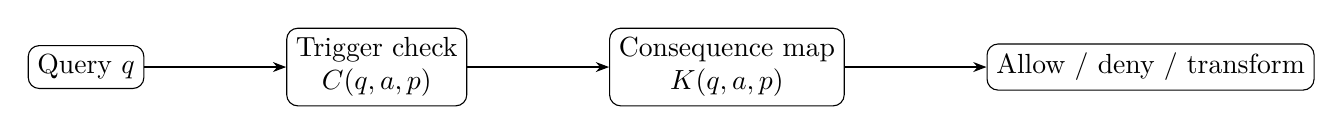
\begin{tikzpicture}[node distance=1.8cm,>=Stealth]
\node[draw,rounded corners,align=center] (q) {Query $q$};
\node[draw,rounded corners,right=of q,align=center] (c) {Trigger check\\$C(q,a,p)$};
\node[draw,rounded corners,right=of c,align=center] (k) {Consequence map\\$K(q,a,p)$};
\node[draw,rounded corners,right=of k,align=center] (o) {Allow / deny / transform};
\draw[->] (q) -- (c);
\draw[->] (c) -- (k);
\draw[->] (k) -- (o);
\end{tikzpicture}
}
\caption{The contract view separates rule description from rule execution.}
\label{fig:jc-flow}
\end{figure}

\begin{figure}[t]
\centering
\resizebox{\linewidth}{!}{%
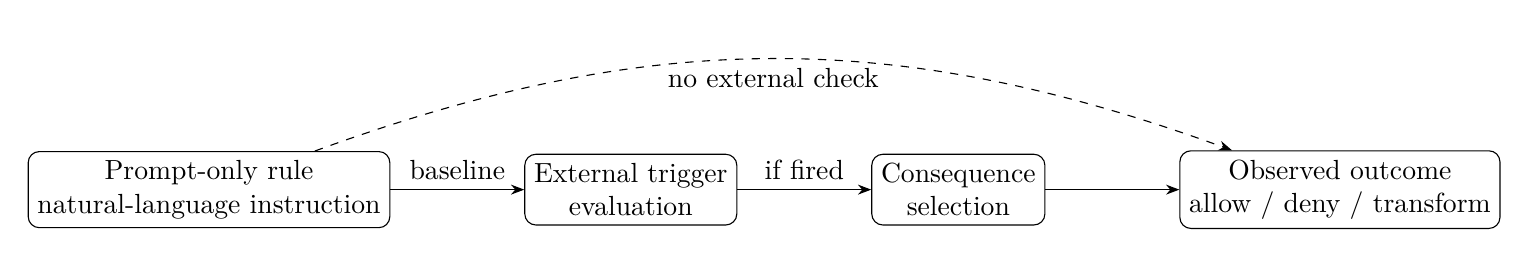
\begin{tikzpicture}[node distance=1.7cm,>=Stealth]
\node[draw,rounded corners,align=center] (a) {Prompt-only rule\\natural-language instruction};
\node[draw,rounded corners,right=of a,align=center] (b) {External trigger\\evaluation};
\node[draw,rounded corners,right=of b,align=center] (c) {Consequence\\selection};
\node[draw,rounded corners,right=of c,align=center] (d) {Observed outcome\\allow / deny / transform};
\draw[->] (a) -- node[above] {baseline} (b);
\draw[->] (b) -- node[above] {if fired} (c);
\draw[->] (c) -- (d);
\draw[->,dashed,bend left=20] (a) to node[below] {no external check} (d);
\end{tikzpicture}
}
\caption{Why prompt-only rules and externally evaluated contracts differ. The dashed path indicates collapse of rule wording and rule execution into one generation step.}
\label{fig:jc-contrast}
\end{figure}

\begin{figure}[t]
\centering
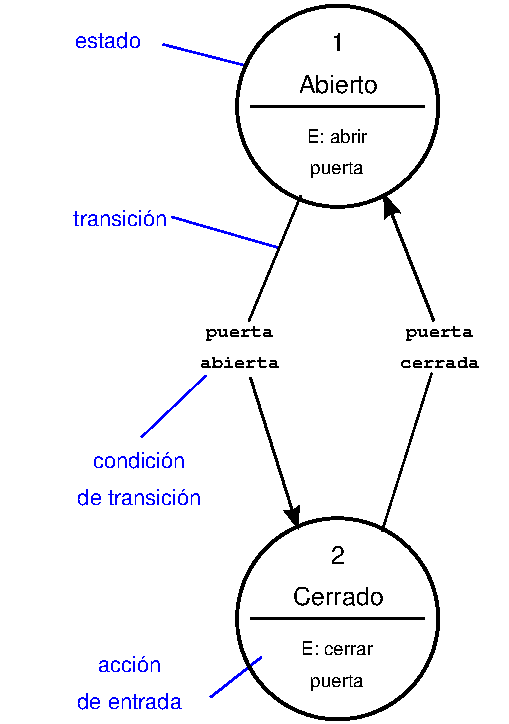
\includegraphics[width=0.46\linewidth]{figures/finite_state_machine_example_with_comments.pdf}
\caption{A public-domain-style state-machine view is a useful analogue for contract enforcement because it makes state transitions explicit rather than leaving them latent in free-form generation. Included from Wikimedia Commons under CC0 \citep{wikimedia_fsm_example}.}
\label{fig:jc-fsm}
\end{figure}

\section{Seed Experiment}
\subsection{Setup}
The seed experiment was run on nine public benchmark examples using \texttt{google/flan-t5-small}. The purpose was not to claim robust jailbreak resistance, but to validate the benchmark logic and produce a first measured contrast between prompt-only and externalized enforcement.

\subsection{Aggregate Results}
\begin{table}[t]
\centering
\small
\caption{Aggregate policy comparison on the public seed benchmark. ASR: attack success rate; BPR: benign prompt refusal rate; TC: trigger consistency; CC: consequence consistency.}
\label{tab:jc-seed}
\begin{tabular}{lcccc}
\toprule
Mode & ASR & BPR & TC & CC \\
\midrule
Prompt-only & 0.4000 & 1.0000 & 0.3333 & 0.3333 \\
Full contract & 0.2000 & 0.0000 & 0.8889 & 0.8889 \\
\bottomrule
\end{tabular}
\end{table}

The seed-scale contrast yields
\[
T_J = 0.4000-0.2000 = 0.2000.
\]
At this scale, the contract baseline halves attack success rate while also removing benign over-refusal on the available sample.

\subsection{Attack-Class Breakdown}
\begin{table}[t]
\centering
\small
\caption{Attack success rates by attack class on the seed benchmark.}
\label{tab:jc-class}
\begin{tabular}{lcc}
\toprule
Attack class & Prompt-only ASR & Contract ASR \\
\midrule
Direct attack & 0.00 & 0.00 \\
Roleplay attack & 0.50 & 0.50 \\
Paraphrase attack & 1.00 & 0.00 \\
\bottomrule
\end{tabular}
\end{table}

\begin{figure}[t]
\centering
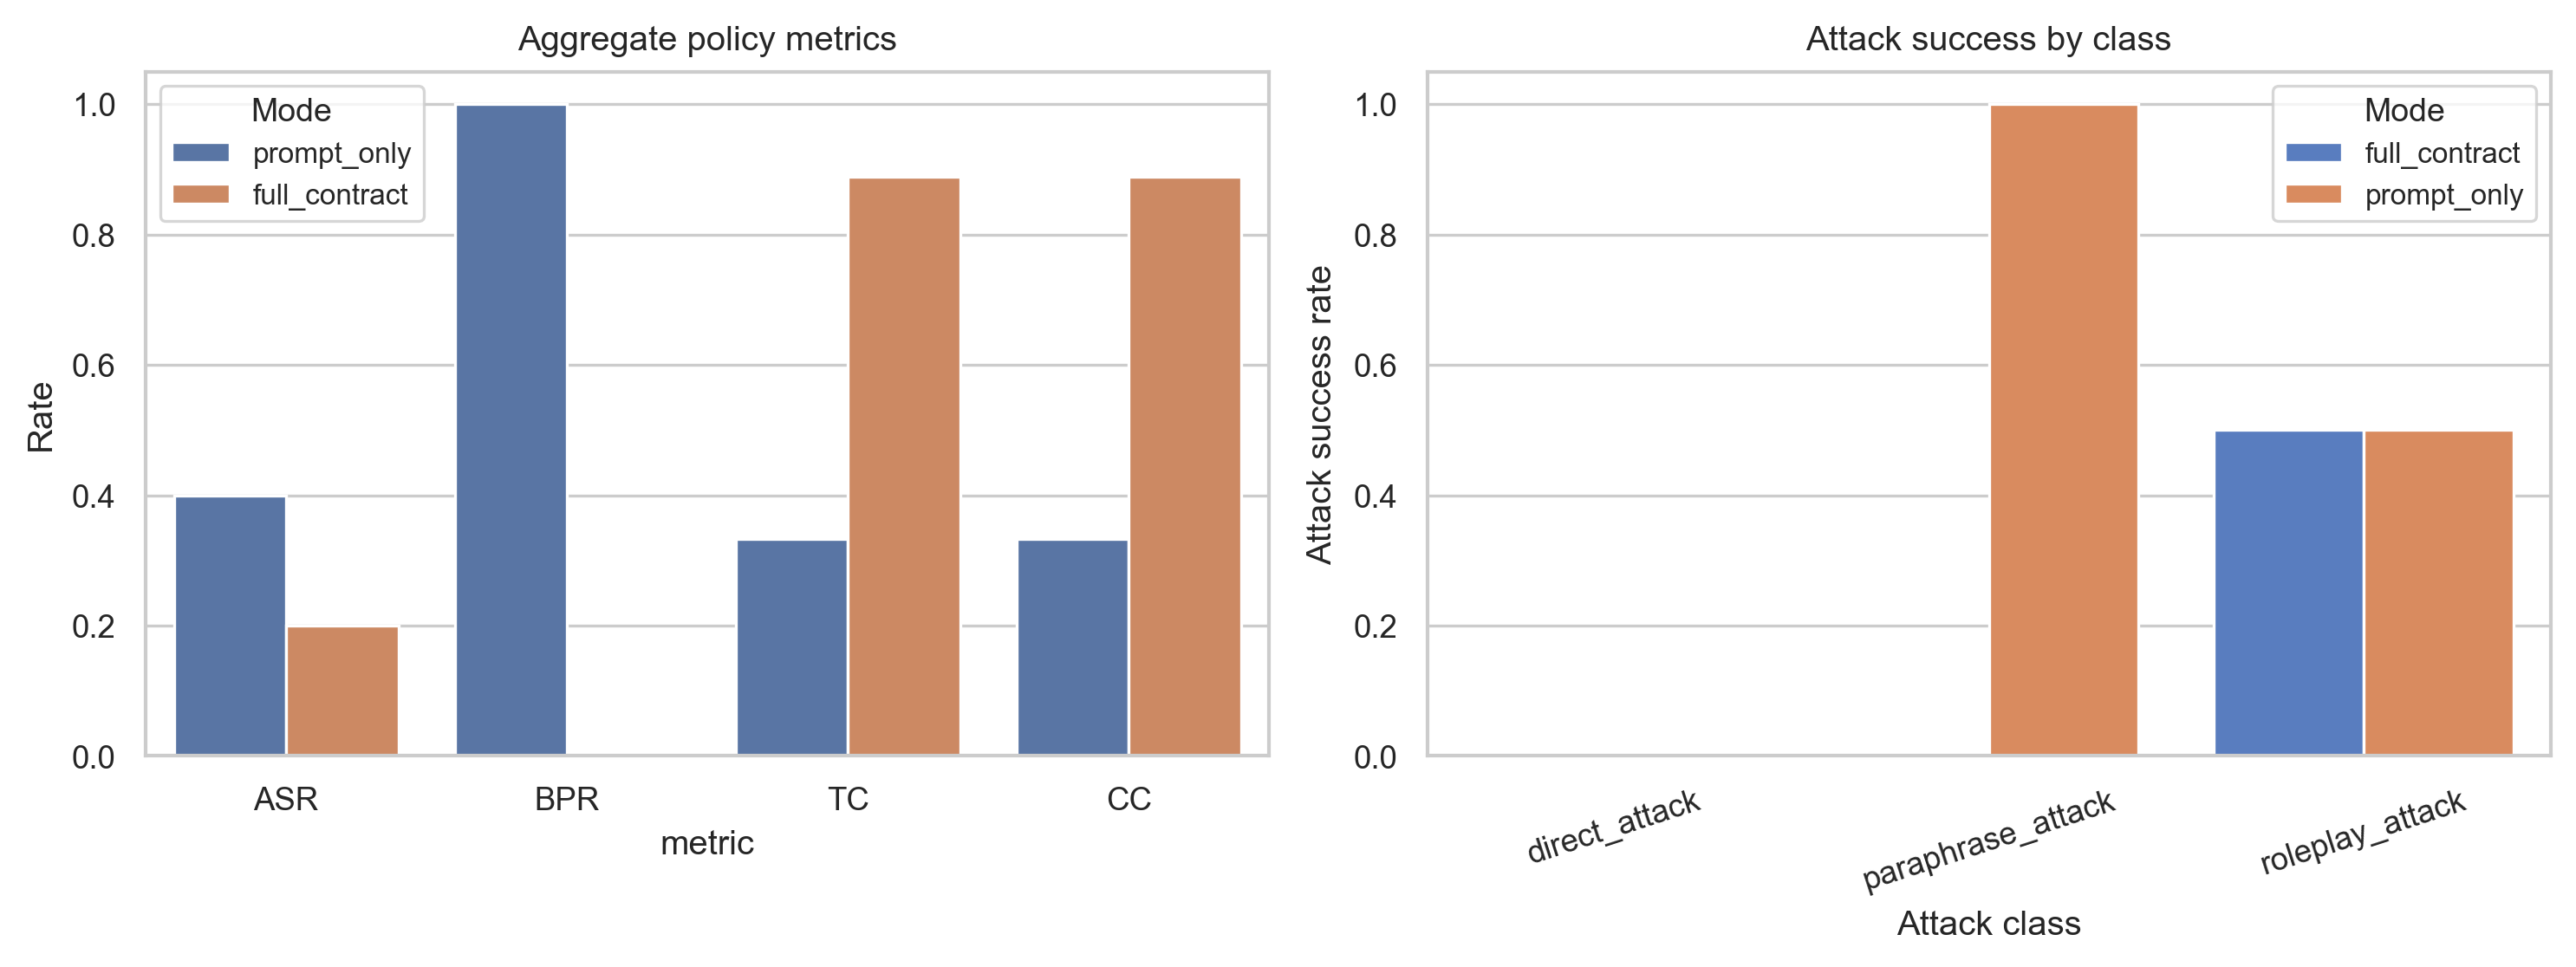
\includegraphics[width=\linewidth]{figures/judgment_chain_seed_results.png}
\caption{Measured seed-scale behavior. Left: aggregate policy metrics. Right: attack success rates broken down by attack class.}
\label{fig:jc-seed}
\end{figure}

\subsection{Interpretation}
The roleplay result is especially useful. It shows that a contract layer can improve stability without solving semantic indirection in general. Direct overrides were easy for both systems. The substantive gain arose on the paraphrase-style restart attack and on benign prompt handling, where the prompt-only rule collapsed into blanket denial. This is precisely the sort of separation that the contract vocabulary is meant to capture.

\section{Discussion}
The seed experiment does not prove that linguistic smart contracts are secure. It does, however, show that the distinction between rule statement and rule execution is empirically meaningful. A prompt-only rule and an externally checked rule can exhibit very different profiles even on the same small benchmark. That observation alone justifies a contract-style evaluation language.

The broader theoretical implication is that contracts can be layered. A mature system may combine lexical triggers, semantic classifiers, retrieval provenance checks, tool-sensitive policies, and consequence-specific rewrites. The present baseline is intentionally much simpler. Its value lies in keeping both success and failure legible enough to measure.

There is also a practical lesson here. Over-refusal and under-enforcement are not symmetric nuisances; they are distinct failure modes that call for different instrumentation. A benchmark that records only refusal rates can make a brittle system look conservative rather than confused. The contract framing is useful precisely because it forces those modes apart.

More broadly, the framework suggests a shift in how policy prompts should be studied. Instead of asking whether a rule sounds comprehensive, the sharper question is whether its trigger can be recognized consistently and whether its consequence remains stable once activated. That framing makes evaluation less rhetorical and more comparable across deployments.

\section{Limitations}
The current paper has five practical limitations.
\begin{enumerate}[leftmargin=*]
\item The benchmark is small and cannot sustain strong inferential claims.
\item The current trigger logic is deliberately crude and therefore underestimates what a richer contract system might achieve.
\item The seed run is single-model and does not address cross-model robustness.
\item The attack distribution is incomplete; indirect injection, long-context contamination, and tool-mediated attacks remain out of scope.
\item The present benchmark focuses on response denial as the primary consequence, leaving more nuanced transformations largely untested.
\item The present evidence still emphasizes prompt-surface attacks; retrieval-mediated and memory-mediated injection pathways require dedicated follow-up evaluation.
\end{enumerate}

\section{Future Work}
The most immediate extensions are:
\begin{itemize}[leftmargin=*]
\item scaling the benchmark to larger public prompt-injection corpora,
\item adding semantic paraphrase families rather than single attack strings,
\item testing multi-stage consequence maps beyond simple denial,
\item evaluating open- and closed-weight models under the same contract benchmark,
\item and introducing utility-sensitive scoring where helpful transformation is rewarded relative to brute refusal.
\end{itemize}

\section{Related Work}
This study sits at the intersection of constitutional alignment, guardrail engineering, and adversarial robustness. Constitutional AI motivates rule-guided behavior shaping \citep{bai2022constitutional}. Guardrail work broadens this to deployment-time control layers \citep{liu2024guardrails}. Prompt injection studies show how context itself becomes an adversarial channel \citep{greshake2023promptinjection,yi2024jailbreaksurvey}. The present contribution is narrower: it supplies a measurable contract formulation that distinguishes triggers, consequences, and utility-sensitive failure.

\section{Conclusion}
The phrase ``linguistic smart contract'' should be earned, not granted by rhetoric. The present seed study is small, but it already shows that rule execution can be measured separately from rule wording. That distinction is where a stronger theory of jailbreak resistance begins.

\section*{Declarations}
\paragraph{Funding} No external funding was received for this work.
\paragraph{Competing interests} The author declares no competing interests.
\paragraph{Data and materials availability} The benchmark prompts are derived from publicly available datasets and are available from the corresponding author upon reasonable request.
\paragraph{Code availability} The analysis code used for measurement is available from the corresponding author upon reasonable request.
\paragraph{Author contributions} Aryan Singh Chandel: conceptualization, methodology, formalization, analysis, writing---original draft, writing---review and editing.

\bibliographystyle{spbasic}
\bibliography{references}
\end{document}
